\chapter{Discussion}
Please tell more about conclusion and how to the next work of this study.

\section{Cokro Edi Prawiro / 1164069}
\subsection{Teori}

\begin{enumerate}

\item Jelaskan Kenapa file teks harus dilakukan tokenizer. Dilengkap dengan ilustrasi atau gambar.\par
Tokenizer adalah proses untuk membagi kalimat menjadi beberapa teks, hal ini sangat di perlukan dalam AI karena nanti setiap teks akan di hitung bobotnya dang akan memunculkan nilai vektor sehingga teks tersebut bisa di gunakan sebagai data untuk memprediksi teks yang muncul dalam satu kalimat sedangakan proses tkenizer merupakan caramembagi bagi teks dari suatu kalimat biasanya pembagi kalimat tersebut merupakan spasi dalan suatu kalimat. Agar lebih jelas dapat melihat gamabr \ref{c131} berikut. 

\begin{figure}[!htbp]
      \centering{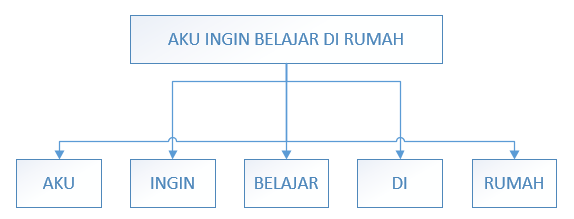
\includegraphics[width=0.7\textwidth]
      {figures/cokro/c131}}
      \caption{Ilustrasi Tokenisasi}
      \label{c131}
      \end{figure}

\item jelaskan konsep dasar K Fold Cross VAlidation dan dataset komentar youtube pada code berikut dilengkapi dengan ilustrasi gambar  
\begin{verbatim}
kfold = StartifiedKFlod(n_splits=5)
splits = kfold.split(d, d['CLASS'])
\end{verbatim}
pada codingan tersebut terdapat kfold sebagai variabel yang didalammnya terdiri dari split 5 yang berarti pengulangan terhadap pengolahan masing masing lima kali pada kasus ini terdapat data sebanyak 5 berarti ke lima data tersebut di ulang sebanyak lima kali dengan atribut class sebagai acuan pengolahan datanya kemudian akan di hasilkan akurasi dari pengulangan data tersebut sebesar sekian persen tergantung datanya. agar lebih jelas dapat di lihat pada gambar \ref{c132}  berikut:

\begin{figure}[!htbp]
      \centering{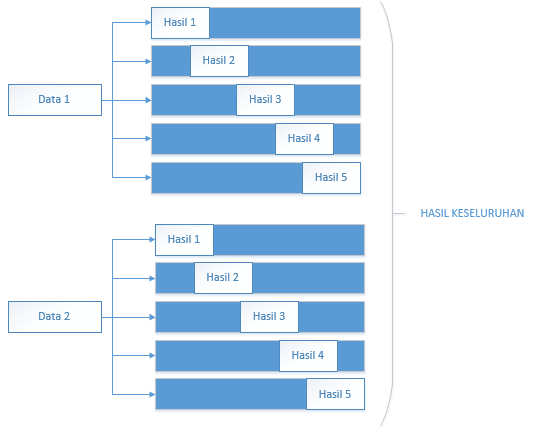
\includegraphics[width=0.7\textwidth]
      {figures/cokro/c132}}
      \caption{Ilustrasi K Fold Cross Validation}
      \label{c132}
      \end{figure}

\item Jelaskan apa maksudnya kode program for train, test in split dilengkapi di lengkapi dengan ilustrasi atau gambar.\par
for train di gunakan melakukan training atau pelatihan terhadap data yang telah di deklarasikan sebelumnya. sedangkan test in split di gunakan untuk diguanakan untuk membatasi jumlah data yang akan di inputkan atau data yang akan di gunakan.agar lebih jelas dapat di lihat pada gambar \ref{c133} berikut.

\begin{figure}[!htbp]
      \centering{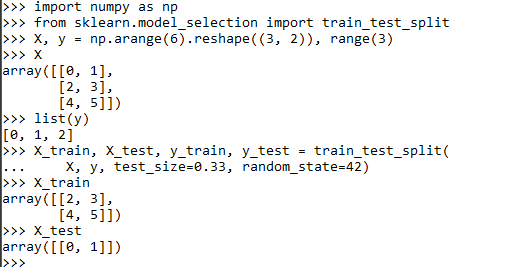
\includegraphics[width=0.7\textwidth]
      {figures/cokro/c133}}
      \caption{Ilustrasi For Train dan Test in split}
      \label{c133}
      \end{figure}

\item Jelaskan apa maksud kode program traint\_content =d['CONTENT'].iloc[traint\_idx] dan test\_content =d['CONTENT'].iloc[traint\_idx]. dilengkapi dengan ilustrasi atau gambar.\par
maksud dari kode program tersebut adalah membaca isian kolom pada field yang bernama CONTENT sebagai data training dan data testing untuk program tersebut sebagai ilustrasi dapat di lihat pada gambar \ref{c134} berikut.

\begin{figure}[!htbp]
      \centering{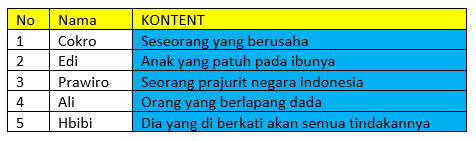
\includegraphics[width=0.7\textwidth]
      {figures/cokro/c134}}
      \caption{Ilustrasi Penggunaan kolom CONTENT}
      \label{c134}
      \end{figure}

\item Jelaskan maksud dari fungsi tokenizer = Tokennizer(num\_words=2000)dan tokenizer.fit\_on\_texts(train\_konten) di lengkapi dengan ilustrasi gambar.\par
fungsi tokenizer = Tokennizer(num\_words=2000) digunakan untuk membaca kalimat yang telah di buat menjadi token sebanyak 2000 kata dan fingsi fit\_on\_texts(train\_konten) digunakan untuk membuat membaca data token teks yang telah di masukan kedalam fungsi yaitu fungsi train\_konten. agar lebih jelas dapat di lihat pada gambar \ref{c135} berikut.

\begin{figure}[!htbp]
      \centering{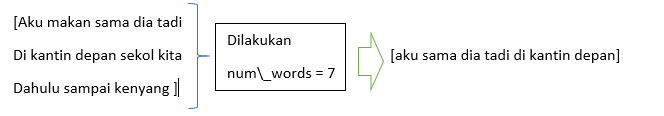
\includegraphics[width=0.7\textwidth]
      {figures/cokro/c135}}
      \caption{Ilustrasi fit tokenizer dan num\_word=2000}
      \label{c135}
      \end{figure}

\item Jelaskan apa maksud dari fungsi d train inputs = tokenizer.texts to matrix(train content, mode=tfidf) dan d test inputs = tokenizer.texts to matrix(test content, mode=tfidf), dilengkapi dengan ilustrasi kode dan atau gambar.\par 
yaitu di gunakan untuk mengubah urutan teks yang tadi telah di lakukan tokenizer menjadi matriks yang berut=rutan seperti tf idf 
contoh seperti gambar \ref{c136} berikut.

\begin{figure}[!htbp]
      \centering{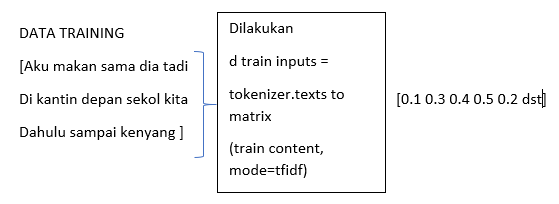
\includegraphics[width=0.7\textwidth]
      {figures/cokro/c136}}
      \caption{Ilustrasi d train inputs = tokenizer.texts to matrix(train content, mode=tfidf)}
      \label{c136}
      \end{figure}

\item Jelaskan apa maksud dari fungsi \emph{d\_train\_inputs = d\_train\_inputs/np.amax(np.absolute(d\_train\_inputs))} dan \emph{d\_test\_inputs = d\_test\_inputs/np.amax(np.absolute(d\_test\_inputs))}, dilengkapi dengan ilustrasi atau gambar \par

fungsi tersebut digunakan untuk membagi matriks tfidf dengan dengan penentuan maksimum aray sepanjang sumbu sehingga akan menimbulkan garis ke bawah dan keatas yang membentuk gambar v kemudian hasil tersebut akan di masukan ke dalam variabel d train input dan d test input dengan methode absolute. yang berarti tanpa bilangan negatif. untuk lebih jelasnya dapat di lihat pada gambar \ref{c137}  berikut ini.

\begin{figure}[!htbp]
      \centering{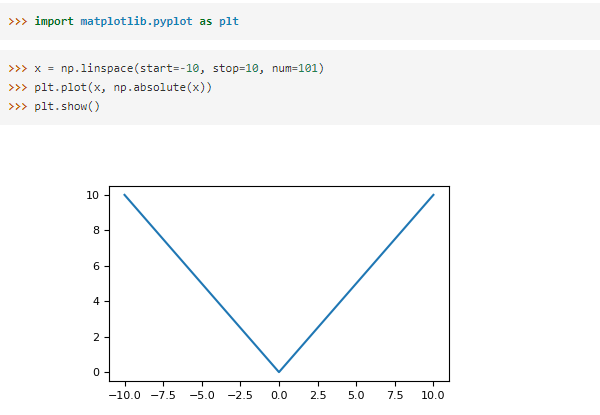
\includegraphics[width=0.7\textwidth]
      {figures/cokro/c137}}
      \caption{Ilustrasi d\_train\_inputs = d\_train\_inputs/np.amax(np.absolute(d\_train\_inputs))}
      \label{c137}
      \end{figure}

\item Jelaskan apa maksud fungsi dari d train outputs = np utils.to categorical(d['CLASS'].iloc[train dan d test outputs = np utils.to categorical(d['CLASS'].iloc[test idx]) dalam kode program, dilengkapi dengan ilustrasi atau gambar.\par

maksud dari fungsi tersebut yaitu untuk merubah nilai vektor yang ada pada atribut class menjadi bentuk matrix dengan pengurutan berdasarkan data index training dan testing. Sebagai contoh dapat di lihat ilustrasi pada gambar \ref{c138} berikut ini.

\begin{figure}[!htbp]
      \centering{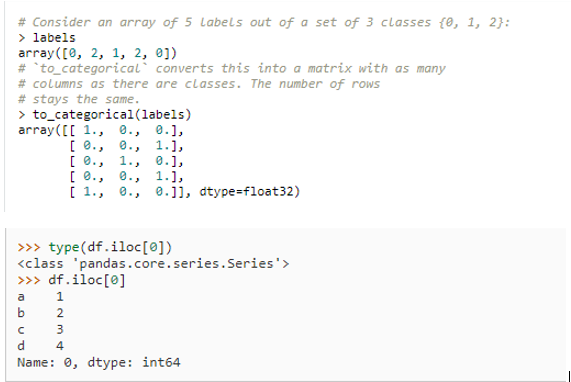
\includegraphics[width=0.7\textwidth]
      {figures/cokro/c138}}
      \caption{Ilustrasid train outputs = np utils.to categorical(d['CLASS'].iloc[train}
      \label{c138}
      \end{figure}

\item model = sequential berarti variabel model berisi method sequential yang berguna untuk searching data dengan menerima parameter atau argumen kunci dengan langkah tertentu untuk mencari data yang telah di olah. kemudian modeldi tambahkan metod add dengan Dense yang berarti data data yang di inputkan akan terhubung, dengan data 612 dan 2000 data  kata atau word kemudian model tersebut di masukan fungsi aktivation dengan rumusa atau methode relu setelah itu data tersebut di dropout 0.5 atau di pangkas sebanyak 50 persen di karenakan pada pohon bobot terlalu akurat terhadap data. sehingga data dilakukan pemangkasan 50 persen. kemudian data tersebut di hubungkan. setelah data tersebut di hubungkan maka di lakukan perhitungan dengan menggunakan fungsi softmax. agar lebih jelas dapat di lihat pada ilustrasi gambar \ref{c139} berikut.

\begin{figure}[!htbp]
      \centering{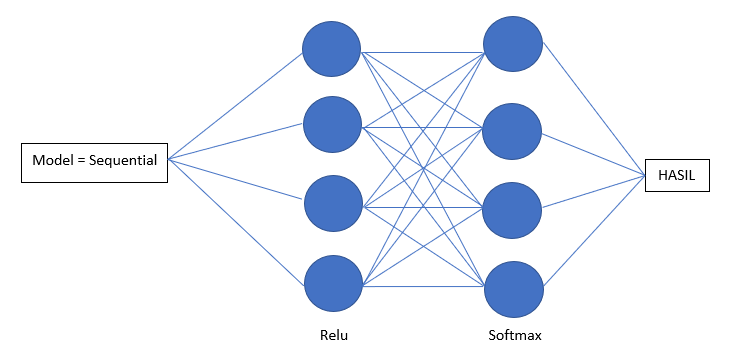
\includegraphics[width=0.7\textwidth]
      {figures/cokro/c139}}
      \caption{Ilustrasid Neural Network}
      \label{c139}
      \end{figure}

\item model tersebut kemudian di compile atau di kembalikan kembali fungsi nilainya yangmana akan mengembalikan fungsi nilai loss nya berapa yang diambil dari fungsi adamax yang berberguna untuk  mengetahui nilai lossnya kemudian metrics = acuracy merupakan akurasi dari nilai matrixnya.

\item Jelaskan apa itu Deep Learning \par
merupakan salah satu algoritma jaringan saraf tiruan yang menggunakan meta data sebagai inputan dan mengolahnya menggunakan layer layer yang tersembunyi. deep lerning memiliki suatu keunikan yaitu fitur yang dapat mengekstraksi secara otomatis.

\item Jelaskan Apa itu Deep Neural Network dan apa perbedaanya dengan Deep Learning.\par
merupakan algoritma jaringan syaraf juga yang mena akan melakukan pembobotan terhadap data yang sudah ada sebagai acuan untuk data inputan selanjutnya. kemudian terdiri atas beberapa layer atau hiden layer. perbedaan antara deep learning dan DNN atau Deep Neural Network yaitu deep lerning merupakan pemakai algoritma dari DNN dan DNN merupakan algoritma yang ada pada deep learning.

\item Jelaskan dengan ilustrasi gambar buatan sendiri(langkah per langkah) bagaimana perhitungan algoritma konvolusi dengan ukuran stride (NPM mod3+1) x (NPM mod3+1) yang terdapat max pooling.(nilai 30)\par
 sebelum membuat ilustrasi perlu di ketahui apa itu stride, stride adalah acuan atau parameter yang menentukan pergeseran pada filter fixcel. sebagai contoh nilai stride 1 yang berarti filter akan bergeser sebanyak satu fixcel secara vertikal dan horizontal. selanjutnya apa itu max pooling contoh pada suatu gambar di tentukan Max Pooling dari 3 x 3 dengan stride 1 yang berarti setiap pergeseran 1 pixcel akan diambil nilai terbesar dari pixcel 3 x 3 tersebut.\par

selanjutnya jawaban dari soal ini yaitu menggunakan stride 1 dengan ketentuan max pooling. untuk jawaban dapat di lihat pada gambar gambar berikut. 

\end{enumerate}

\section{Fathi Rabbani / 1164074}
\subsection{Teori}
\begin{enumerate}
\item Kenapa file Text harus di Tokenizer
\par Tokenizer adalah langkah pertama yang diperlukan dalam tugas pemrosesan bahasa, seperti penghitungan kata, penguraian, pemeriksaan ejaan, pembuatan corpus, dan analisis statistik teks. Itu mengkonversi string teks Python menjadi aliran objek token, di mana setiap objek token adalah kata yang terpisah, tanda baca, nomor / jumlah, tanggal, email, URL / URI, dll. Ini juga mengelompokkan aliran token menjadi kalimat, dengan mempertimbangkan sudut kasus-kasus seperti singkatan dan tanggal di tengah kalimat. ilustrasi dapat dilihat pada Gambar \ref{data1}

\begin{figure}[!htbp]
      \centering{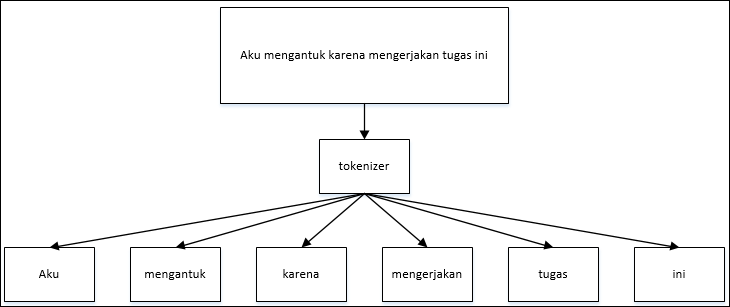
\includegraphics[width=0.6\textwidth]{figures/fathi/chapter7/hari1/1}}
      \caption{Ilustrasi Tokenisasi}
      \label{data1}
\end{figure}

\item Konsep dasar K Fold Cross Validation pada dataset Komentar Youtube

\begin{lstlisting}[caption=K Fold Cross Validation,label={lst:1}]
kfold = StratifiedKFold(n_splits=5)
splits = kfold.split(d, d['CLASS'])
\end{lstlisting}

\par pada Code pada Listing \ref{lst:1} terdapat penggunaan K Fold dengan metode yang akan membagi data dalam 5 hasil pengulangan dari pembagian data yang akan dilakukan pada Attribute CLASS. ilustrasinya dapat dilihat pada Gambar \ref{data2}

\begin{figure}[!htbp]
      \centering{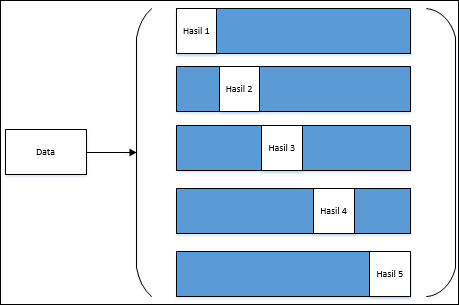
\includegraphics[width=0.6\textwidth]{figures/fathi/chapter7/hari1/2}}
      \caption{Ilustrasi  K Fold Cross Validation pada dataset Komentar Youtube}
      \label{data2}
\end{figure}

\item Jelaskan apa maksudnya kode program \emph{for train, test in splits}
\par Membagi susunan atau matriks menjadi rangkaian acak, dimana data yang dimasukan akan dibagi dengan porsi yang sesuai dengan Train dan Test datanya. untuk lebih jelas tentang bagaimana penggunaannya dapat dilihat pada Gambar \ref{data3}

\begin{figure}[!htbp]
      \centering{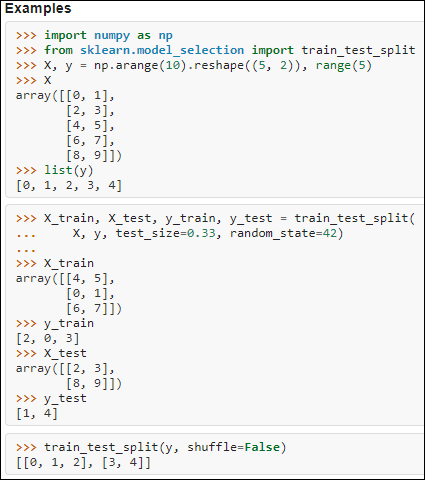
\includegraphics[width=0.6\textwidth]{figures/fathi/chapter7/hari1/3}}
      \caption{Ilustrasi  penggunaan Train dan Test Split}
      \label{data3}
\end{figure}

\item Maksud Code program \emph{train\_content = d['CONTENT'].iloc[train\_idx]} dan \emph{test\_content = d['CONTENT'].iloc[train\_idx]}
\par pada code tersebut dimaksudkan untuk membaca data isian yang terdapat pada kolom yang bernama attributenya CONTENT sebagai data TRAIN dan data TEST, untuk ilustrasinya dapat dilihat pada Gambar \ref{data4}

\begin{figure}[!htbp]
      \centering{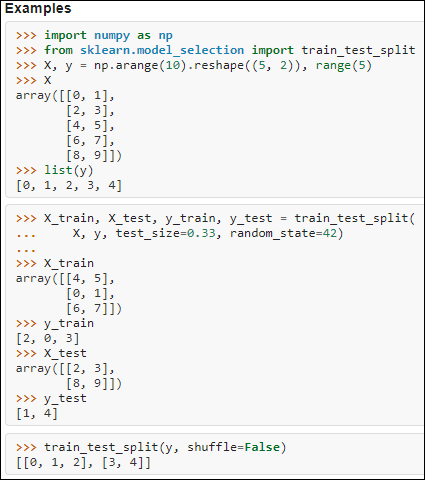
\includegraphics[width=0.6\textwidth]{figures/fathi/chapter7/hari1/3}}
      \caption{Ilustrasi  penggunaan Train dan Test Split}
      \label{data4}
\end{figure}

\item maksud dari fungsi \emph{tokenizer = Tokenizer(num\_words=2000)} dan \emph{tokenizer.fit\_on\_texts(train\_content)}
\par pada code tersebut dimana penggunaan Tokenizer berguna untuk membaca data teks yang berformat kalimat untuk disusun sebanyak 2000 kata, fungsi fit\_on\_texts(train\_content) untuk membaca data Teks Tokenizer tadi untuk dimasukan kedalam kolom CONTENT pada dataset. untuk contoh ilustrasi data yang digunakan dapat dilihat pada Gambar \ref{data5}

\begin{figure}[!htbp]
      \centering{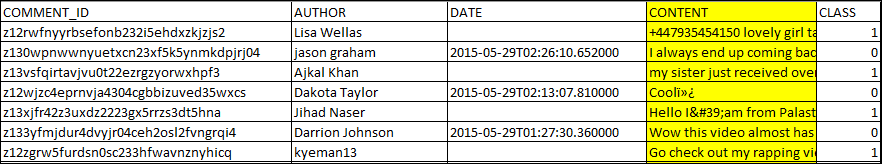
\includegraphics[width=0.6\textwidth]{figures/fathi/chapter7/hari2/1}}
      \caption{data Content yang dimaksud}
      \label{data5}
\end{figure}

\item maksud dari fungsi \emph{d\_train\_inputs = tokenizer.texts\_to\_matrix(train\_content, mode='tfidf')} dan \emph{d\_test\_inputs = tokenizer.texts\_to\_ matrix(test\_content, mode='tfidf')}

\par pada code yang pertama terdapat fungsi yang digunakan untuk mengolah data variable d\_train\_inputs dan d\_test\_inputs dengan menggunakan tokernizer dengan fungsi yang merubah data teks menjadi data matrix dengan pemrosesan datanya sesuai dengan data Variable train\_content dan test\_content dengan metodenya adalah TF-IDF. untuk contoh ilustrasi dari penjelasan tersebut dapat dilihat pada Gambar \ref{data6}

\begin{figure}[!htbp]
      \centering{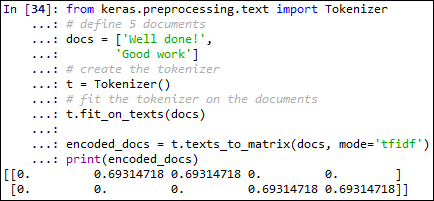
\includegraphics[width=0.6\textwidth]{figures/fathi/chapter7/hari2/2}}
      \caption{Contoh code tentang penggunaan texts\_to\_matrix}
      \label{data6}
\end{figure}

\item maksud dari fungsi \emph{d\_train\_inputs = d\_train\_inputs/np.amax(np.absolute(d\_train\_inputs))} dan \emph{d\_test\_inputs = d\_test\_inputs/np.amax(np.absolute(d\_test\_inputs))}

\par pada code tersebut berfungsi sebagai pengelolaan data Variable d\_train\_inputs dan d\_test\_inputs dengan menggunakan perintah metode yang terdapat pada Library Numpy metode yang diggunakan adalah AMAX yang berguna untuk mengambil nilai maksimum yang terdapat pada data arraynya atau mencari nilai maksimum dari panjang sumbu yang terproses dan ABSOLUTE yang berguna untuk untuk mengkalkulasi nilai pasti dari setiap data elemennya. untuk contoh dari pengguaan AMAX dan ABSOLUTE dapat dilihat pada Gambar \ref{data7} dan Gambar \ref{data8}

\par berikut ini adalah contoh Code yang digunakan untuk menjelaskan penggunaan AMAX :
\begin{figure}[!htbp]
      \centering{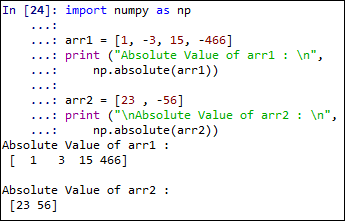
\includegraphics[width=0.6\textwidth]{figures/fathi/chapter7/hari2/3}}
      \caption{penggunaan Numpy AMAX}
      \label{data7}
\end{figure}

\par berikut ini adalah contoh Code yang digunakan untuk menjelaskan penggunaan ABSOLUTE :
\begin{figure}[!htbp]
      \centering{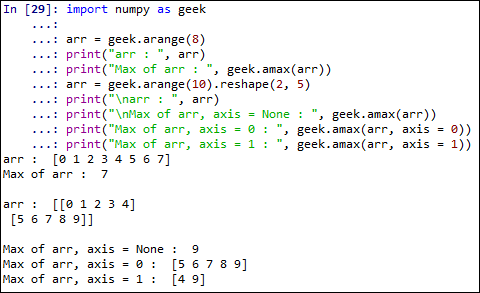
\includegraphics[width=0.6\textwidth]{figures/fathi/chapter7/hari2/4}}
      \caption{penggunaan Numpy ABSOLUTE}
      \label{data8}
\end{figure}

\item maksud fungsi dari \emph{d\_train\_outputs = np\_utils.to\_categorical(d['CLASS'].iloc[train\_idx])} dan \emph{d\_test\_outputs = np\_utils.to\_categorical(d['CLASS'].iloc[test\_idx])} dalam kode program

\par pada code tersebut menjelaskan penggunaan Library Numpy yang akan mengelola data d\_train\_outputs dan d\_test\_outputs dengan menggunakan perintah atau metode TO\_CATEGORICAL dimana data yang diambil adalah data CLASS dengan index data yang dituju adalah train\_idx dan test\_idx, dimana to\_categorical berguna untuk mengkonversikan data kelas Vektor(Integer) menjadi data kelas Binary Matrix. contoh penggunaan to categorical dapat dilihat pada Gambar \ref{data9}

\begin{figure}[!htbp]
      \centering{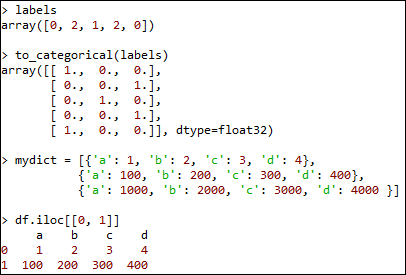
\includegraphics[width=0.6\textwidth]{figures/fathi/chapter7/hari2/5}}
      \caption{Contoh Code dan Hasil dari penggunaan to\_categorical dan iloc}
      \label{data9}
\end{figure}

\item Penjelasan pada fungsi code dengan Ilustrasi Neural Networknya
\begin{lstlisting}[caption=Membuat model Neural Network,label={lst:2}]
       model = Sequential()
       model.add(Dense(512, input_shape=(2000,)))
       model.add(Activation('relu'))
       model.add(Dropout(0.5))
       model.add(Dense(2))
       model.add(Activation('softmax'))
\end{lstlisting}
\par pada code yang terdapat pada  Listing \ref{lst:3}, dijelaskan bahwa dibuatkannya Variable 'model' untuk menampung model Sequential() atau metode yang berguna untuk menumpuk data Linear. berikut ini adalah  penjelasan dari masing - masing fungsi yang terdapat pada Code tersebut :
\begin{itemize}
\item Dense (512, input\_shape = (2000,)) dan (2)
\par dimana data yang diolah akan berjumlah 512 dengan shape yang diolah dalah 2000 begitu juga dengan yang 2

\item Activation ('relu') dan ('softmax')
\par Activation adalah untuk melakukan penggunaan fungsi matematika, relu yang berarti fungsi dari metode 'Rectified Linear Unit' dan softmax yang berguna untuk menghasilkan data Vector yang merepresentasikan nilai distibusi probabilitas dari daftar nl=ilai output yang memiliki potensi.

\item Dropout(0.5)
\par melakukan set sebanyak 50 persen pada output atau nilai hasil yang dikeluarkan dari pengelolaan data pada visible layer dan hidden layer.
\end{itemize}
\par berikut ini adalah contoh dari struktur Neural Network yang terjadi :
\begin{figure}[!htbp]
      \centering{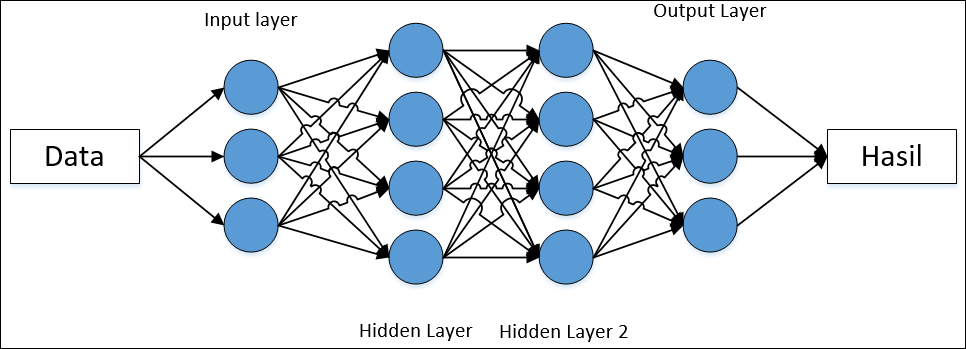
\includegraphics[width=0.6\textwidth]{figures/fathi/chapter7/hari2/7}}
      \caption{Contoh dari struktur Neural Network yang terjadi}
      \label{data10}
\end{figure}

\item Maksud dari fungsi pada Code berikut :
\begin{lstlisting}[caption=Compile model,label={lst:3}]
	model.compile(loss='categorical_crossentropy', optimizer='adamax',
	                  metrics=['accuracy'])
\end{lstlisting}
\par pada code tersebut menjelaskan tentang proses yang berlangsung untuk menampilkan nilai LOSS dan ACCURACY yang dihasilkan dari Compile pada program diatas.

\item Jelaskan apa itu Deep Learning
\par Deep Learning adalah rangkaian metode untuk bisa melatih jaringan saraf buatan multi lapisan atau mempunyai banyak lapisan. Metode ini sangat efektif dan lebih mudah dalam mengidentifikasi pola dari data yang dimasukkan. Deep Learning juga dapat meningkatkan bagian AI, mulai dari memproses bahasa alami yang kita katakana sampai dengan mengambil gambar. Oleh karena itu Deep Learning merupakan otak yang lebih baik dan unggul untuk meningkatkan cara kerja pada sistem komputer

\item Jelaskan Apa itu Deep Neural Network dan apa perbedaanya dengan Deep Learning
\par Deep Neural Network adalah Neural Network dengan tingkat kompleksitas tertentu, Neural Network dengan lebih dari dua lapisan.  Neural Network dalam menggunakan pemodelan matematika yang canggih untuk memproses data dengan cara yang kompleks. perbedaan antara Deep Learning dan DNN adalah DNN merupakan sebuah Algoritma yang terdapat dalam Deep Learning itu sendiri sedangkan Deep Learning adalah sebuah pengguna dari algoritma pada DNN.

\item Jelaskan dengan ilustrasi gambar buatan sendiri(langkah per langkah) bagaimana perhitungan algoritma konvolusi dengan ukuran stride (NPM mod3+1) x (NPM mod3+1) yang terdapat max pooling

\par Konvolusi terdapat pada operasi pengolahan citra yang mengalikan sebuah citra dengan sebuah mask atau kernel, Stride adalah parameter yang berfungsi untuk menentukan pergeseran pada filter data pixel yang terjadi. untuk contoh penggunaannya dapat dilihat pada Gambar \ref{data11}

\begin{figure}[!htbp]
      \centering{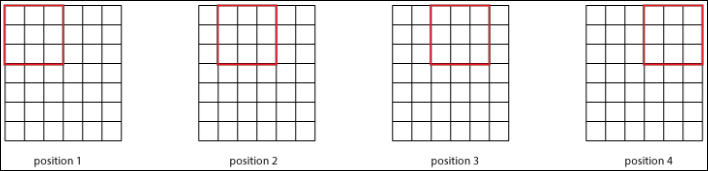
\includegraphics[width=0.6\textwidth]{figures/fathi/chapter7/hari2/6}}
      \caption{Penggunaan Konvolusi dengan Stridenya adalah 3 x 3}
      \label{data11}
\end{figure}

\end{enumerate}


\subsection{Pemrograman}
\begin{enumerate}
\item 
\end{enumerate}